\documentclass{article}
\usepackage[T1]{fontenc}
\usepackage{lmodern}
\usepackage{graphicx}
\usepackage{amsmath,amssymb}
\usepackage[a4paper,margin=2cm]{geometry}
\usepackage[absolute,overlay]{textpos}
\setlength{\TPHorizModule}{1mm}
\setlength{\TPVertModule}{1mm}
\usepackage[indonesian]{babel}
\usepackage{hyperref}
\setlength{\emergencystretch}{2em}
% unit: Halaman 8

\begin{document}

% === Halaman 8 (llm) ===

\textbf{Niels Henrik Abel} (5 August 1802 -- 6 April 1829) was a \href{https://en.wikipedia.org/wiki/Norwegian}{Norwegian} \href{https://en.wikipedia.org/wiki/Mathematician}{mathematician} who made pioneering contributions in a variety of fields. His most famous single result is the first complete proof demonstrating the impossibility of solving the \href{https://en.wikipedia.org/wiki/Quintic_equation}{general quintic equation} in radicals. This question was one of the outstanding open problems of his day, and had been unresolved for 250 years. He was also an innovator in the field of \href{https://en.wikipedia.org/wiki/Elliptic_function}{elliptic functions}, discoverer of \href{https://en.wikipedia.org/wiki/Abelian_function}{Abelian functions}. Despite his achievements, Abel was largely unrecognized during his lifetime; he made his discoveries while living in poverty and died at the age of 26.

Most of his work was done in six or seven years of his working life.\cite{1} Regarding Abel, the French mathematician \href{https://en.wikipedia.org/wiki/Charles_Hermite}{Charles Hermite} said: "Abel has left mathematicians enough to keep them busy for hundred years.\cite{1}\cite{2}"

\vspace{93.56mm}

Another French mathematician, \href{https://en.wikipedia.org/wiki/Adrien-Marie_Legendre}{Adrien-Marie Legendre}, said: "quelle t\^ete c\^elle du jeune Norv\^egien!" ("what a head the young Norwegian has!")\cite{3}

\vspace{10mm}

\begin{tabular}{ll}
Born & 5 August 1802 \\
& \href{https://en.wikipedia.org/wiki/Nedstrand}{Nedstrand}, \href{https://en.wikipedia.org/wiki/Norway}{Norway} \\
Died & 6 April 1829 (aged 26) \\
& \href{https://en.wikipedia.org/wiki/Froland}{Froland}, \href{https://en.wikipedia.org/wiki/Norway}{Norway} \\
Residence & Norway \\
Nationality & Norwegian \\
Fields & \href{https://en.wikipedia.org/wiki/Mathematics}{Mathematics} \\
Alma mater & \href{https://en.wikipedia.org/wiki/Royal_Frederick_University}{Royal Frederick University} \\
Known for & \begin{itemize}
\item Abel's binomial theorem
\item Abelian category
\item Abelian variety
\item Abelian variety of CM-type
\item Abel equation
\item Abel equation of the first kind
\item Abelian extension
\item Abel function
\item Abelian group
\item Abel's identity
\item Abel's inequality
\item Abel's irreducibility theorem
\item Abel--Jacobi map
\item Abel--Plana formula
\item Abel--Ruffini theorem
\item Abelian means
\item Abel's summation formula
\item Abel's theorem
\item Abel transform
\item Abel transformation
\item Abelian variety
\item Dual abelian variety
\end{itemize}
\end{tabular}

Sumber: Wikipedia

% deskripsi: Foto potret hitam putih Niels Henrik Abel
% bbox normalisasi: [0.4970, 0.3450, 0.6950, 0.6600]
\begin{textblock*}{41.58mm}(104.37mm,102.46mm)
\noindent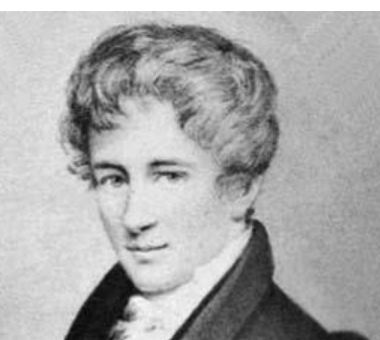
\includegraphics[width=41.58mm,height=93.56mm]{../../images/llm/page_008_img_01.png}%
\end{textblock*}

\end{document}
